\section{Flag 02 - Include}

\paragraph{b12c4b2cb8094750ae121a676269aa9e2872d07c06e429d25a63196ec1c8c1d0}

\begin{center}
    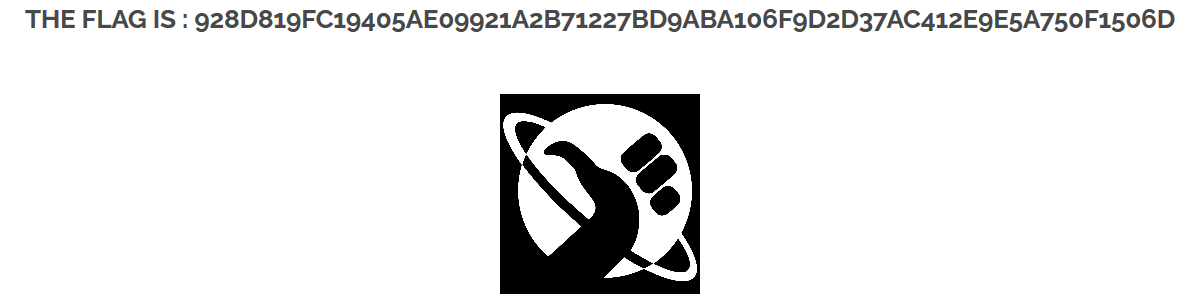
\includegraphics[width=0.5\textwidth]{05.Flag02/02-07.png}\\[0cm] 
\end{center}

\subsection{Vulnerability}

This is a classic attack often refered to as a `Directory Traversal Attack`.

\subsection{Location}

http://<ip-address>:80/index.php?page=../../../../../../../../../etc/passwd

\subsection{Method}

If you open Object Inspection Tool, you will see under the Network Tab that you are able to view the HTTP Headers. The one to look out for is `X-Powered-By PHP/5.3.10-1ubuntu3.19`.

It being `ubuntu` tells us that it is using a Unix File system. Therefore we are looking to see if we can gain access to `etc\\passwd`.

If you check the example on \href{https://en.wikipedia.org/wiki/Directory\_traversal\_attack}{Wikipedia}, the example states:

```

GET /vulnerable.php HTTP/1.0

Cookie: TEMPLATE=../../../../../../../../../etc/passwd

```

so the plan was to see if this will work if I tried to traverse the includes() until reaching the root directory.

This means consistently appending `../` until reaching the root directory.

\subsection{Tools}

\begin{figure}[!htb]
    \centering
    \subfloat[Wtf ?]{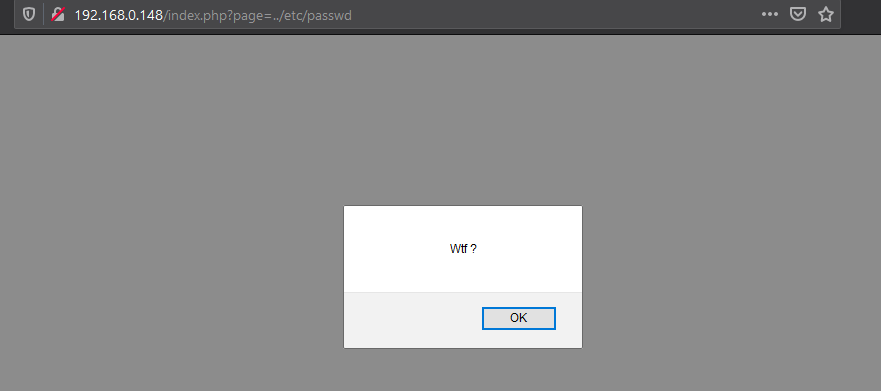
\includegraphics[width=.45\columnwidth]{05.Flag02/02-01.png}\label{fig: 02-01 - wtf}} \quad
    \subfloat[Wrong..]{
\includegraphics[width=.45\columnwidth]{05.Flag02/02-02.png}\label{fig: 02-02 - wrong}} \\
    \subfloat[Nope..]{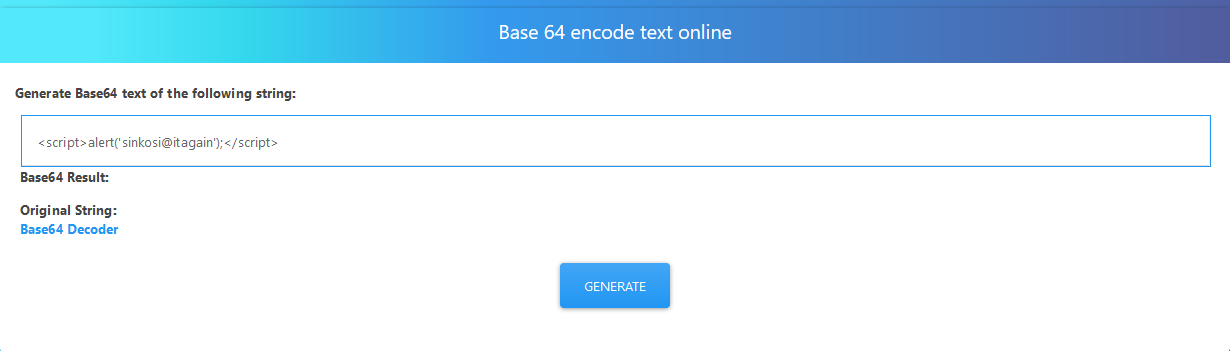
\includegraphics[width=.45\columnwidth]{05.Flag02/02-03.png}\label{fig: 02-03 - nope}} \quad
    \subfloat[Almost]{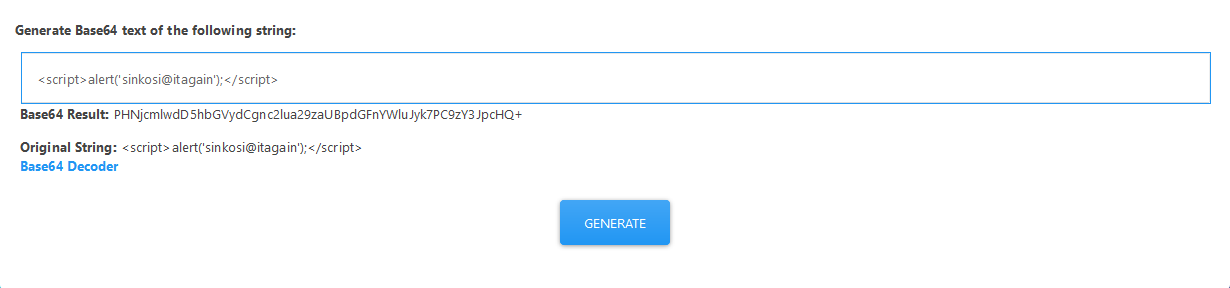
\includegraphics[width=.45\columnwidth]{05.Flag02/02-04.png}\label{fig: 02-04 - almost}}
    \subfloat[Still nope]{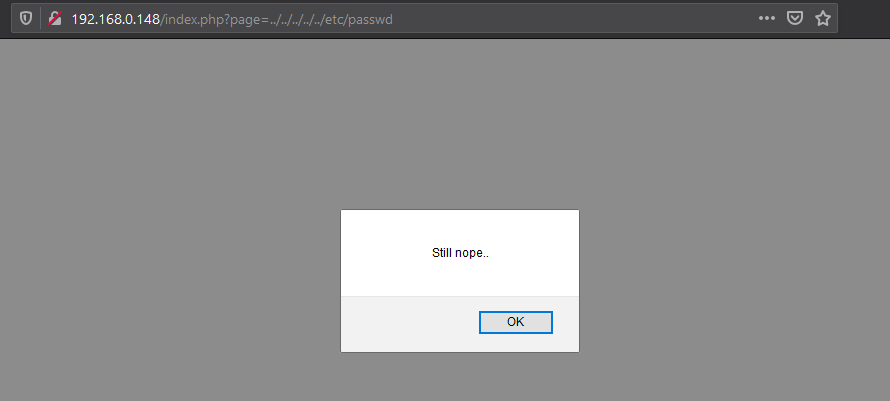
\includegraphics[width=.45\columnwidth]{05.Flag02/02-05.png}\label{fig: 02-05 - still nope}} \quad
    \subfloat[More Nope]{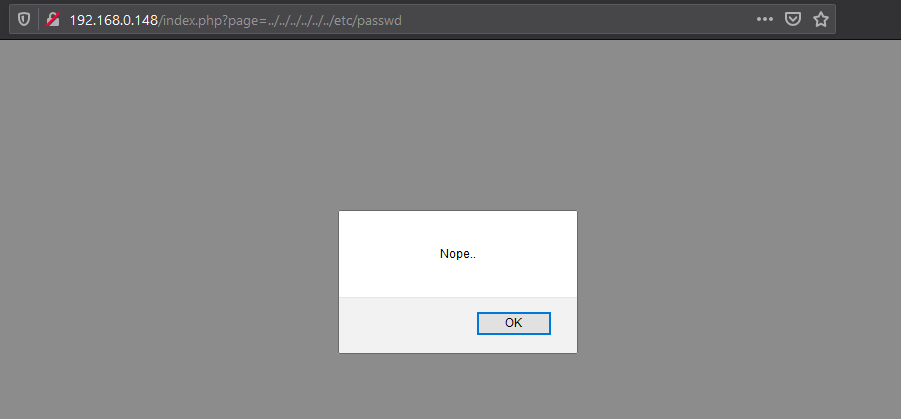
\includegraphics[width=.45\columnwidth]{05.Flag02/02-06.png}\label{fig: 02-06 - Nope..}}
    \caption[Flag 02 Method]{Process to Capture the Include Flag} % The text in the square bracket is the caption for the list of figures while the text in the curly brackets is the figure caption
    \label{fig:flag02 method}
\end{figure}

\begin{itemize}
    \item Mozilla Firefox Inspection Tool
    \item \href{https://en.wikipedia.org/wiki/Directory\_traversal\_attack}{Wikipedia - Directory Traversal Attack}
    \item \href{https://owasp.org/www-community/attacks/Path\_Traversal}{OWASP - Path Traversal}
\end{itemize}

\subsection{Remedy}

\begin{itemize}
    \item Process URI requests that do not result in a file request, e.g., executing a hook into user code, before continuing below.
    \item When a URI request for a file/directory is to be made, build a full path to the file/directory if it exists, and normalize all characters (e.g., %20 converted to spaces).
    \item It is assumed that a 'Document Root' fully qualified, normalized, path is known, and this string has a length N. Assume that no files outside this directory can be served.
    \item Ensure that the first N characters of the fully qualified path to the requested file is exactly the same as the 'Document Root'.
    
    If so, allow the file to be returned.
    If not, return an error, since the request is clearly out of bounds from what the web-server should be allowed to serve.
    
    \item Using a hard-coded predefined file extension to suffix the path does not limit the scope of the attack to files of that file extension.
    
\end{itemize}